\documentclass[12pt,hyperref,a4paper,UTF8]{ctexart}
\usepackage{HDUReport}
\usepackage{listings}
\usepackage{xcolor}
\usepackage{graphicx}
\usepackage{setspace}
\usepackage{float}
\setstretch{1.5} % 设置全局行距为1.5倍

\usepackage{enumitem} % 载入enumitem包以便自定义列表环境
\setlist[itemize]{itemsep=0pt, parsep=0pt} % 设置itemize环境的项目间距和段落间距

\setmainfont{Times New Roman} % 英文正文为Times New Roman


\usepackage{tikz}
\usetikzlibrary{shapes.geometric, arrows}
\usetikzlibrary{positioning, arrows.meta}
\usetikzlibrary{calc}
%封面页设置
{   
    %标题
    \title{ 
        \vspace{1cm}
        \heiti \Huge \textbf{《单片机原理及应用》作业报告} \par
        \vspace{1cm} 
        \heiti \Large {\underline{实验报告5第一部分:锯齿波生成}   } 
        \vspace{3cm}
    
    }

    \author{
        \vspace{0.5cm}
        \kaishu\Large 学院\ \dlmu[9cm]{卓越学院} \\ %学院
        \vspace{0.5cm}
        \kaishu\Large 学号\ \dlmu[9cm]{23040447} \\ %班级
        \vspace{0.5cm}
        \kaishu\Large 姓名\ \dlmu[9cm]{陈文轩} \qquad  \\ %学号
        \vspace{0.5cm}
        \kaishu\Large 专业\ \dlmu[9cm]{智能硬件与系统(电子信息工程)} \qquad \\ %姓名 
    }
        
    \date{\today} % 默认为今天的日期,可以注释掉不显示日期
}
%%------------------------document环境开始------------------------%%
\begin{document}

%%-----------------------封面--------------------%%
\cover
\thispagestyle{empty} % 首页不显示页码
%%------------------摘要-------------%%
%\newpage
%\begin{abstract}




%\end{abstract}

%\thispagestyle{empty} % 首页不显示页码

%%--------------------------目录页------------------------%%
% \newpage
% \tableofcontents
% \thispagestyle{empty} % 目录不显示页码

%%------------------------正文页从这里开始-------------------%
\newpage
\setcounter{page}{1} % 让页码从正文开始编号

%%可选择这里也放一个标题
%\begin{center}
%    \title{ \Huge \textbf{{标题}}}
%\end{center}


\textbf{原题目:DACO832与单片机的接线如课堂上所接,参考电压为-10V,请编程实现锯齿波的波形,锯齿波的周期为20+作业号,单位是ms。}


\section{实验代码}

\begin{lstlisting}[language=C, caption={实验程序}]

#include <reg51.h>
#define DATA P2
#define STUDENT_ID 47   // 学号定义为47

// 波形输出总时间 = (学号 + 20)ms
#define TOTAL_TIME (STUDENT_ID/1.375 + 20)  // 单位:ms
unsigned char mode = 0;  // 0:自定义波形, 1:锯齿波, 2:三角波

// 自定义波形表 - 从+1V到+2V再到0V
// 0V对应值为0,1V对应值为128,2V对应值为255
unsigned char code customWave[256] = {
    // 0-15: 起始点(+1V)到上升过程
    128, 132, 136, 140, 144, 148, 152, 156, 160, 164, 168, 172, 176, 180, 184, 188,
    // 16-31: 继续上升
    192, 196, 200, 204, 208, 212, 216, 220, 224, 228, 232, 236, 240, 244, 248, 252,
    // 32-47: 到达峰值(+2V)并开始下降
    255, 255, 250, 245, 240, 235, 230, 225, 220, 215, 210, 205, 200, 195, 190, 185,
    // 48-63: 继续下降
    180, 175, 170, 165, 160, 155, 150, 145, 140, 135, 130, 125, 120, 115, 110, 105,
    // 64-79: 继续下降
    100, 95, 90, 85, 80, 75, 70, 65, 60, 55, 50, 45, 40, 35, 30, 25,
    // 80-95: 接近0V
    20, 15, 10, 5, 0, 0, 0, 0, 0, 0, 0, 0, 0, 0, 0, 0,
    // 96-111: 保持0V一段时间
    0, 0, 0, 0, 0, 0, 0, 0, 0, 0, 0, 0, 0, 0, 0, 0,
    // 112-127: 开始回升
    5, 10, 15, 20, 25, 30, 35, 40, 45, 50, 55, 60, 65, 70, 75, 80,
    // 128-143: 继续回升
    85, 90, 95, 100, 105, 110, 115, 120, 125, 130, 135, 140, 145, 150, 155, 160,
    // 144-159: 继续回升至起始点(+1V)
    165, 170, 175, 180, 185, 190, 195, 200, 205, 210, 215, 220, 225, 230, 235, 240,
    // 160-255: 保持1V电平直到循环结束
    128, 128, 128, 128, 128, 128, 128, 128, 128, 128, 128, 128, 128, 128, 128, 128,
    128, 128, 128, 128, 128, 128, 128, 128, 128, 128, 128, 128, 128, 128, 128, 128,
    128, 128, 128, 128, 128, 128, 128, 128, 128, 128, 128, 128, 128, 128, 128, 128,
    128, 128, 128, 128, 128, 128, 128, 128, 128, 128, 128, 128, 128, 128, 128, 128,
    128, 128, 128, 128, 128, 128, 128, 128, 128, 128, 128, 128, 128, 128, 128, 128,
    128, 128, 128, 128, 128, 128, 128, 128, 128, 128, 128, 128, 128, 128, 128, 128
};


unsigned int timer_count = 0;  // 定时器计数

// 计算锯齿波数据
unsigned char getSawWave(unsigned char i)
{
    // 锯齿波是线性上升的波形
    return i;  // 值从0线性增加到255
}

// 计算三角波数据
unsigned char getTriangleWave(unsigned char i)
{
    if(i < 128)
        return i << 1;  // 0-255上升段
    else
        return 255 - ((i - 128) << 1);  // 255-0下降段
}

// 定时器0初始化
void Timer0Init()
{
    TMOD = 0x01;    // 设置定时器0为模式1(16位定时器)
    EA = 1;         // 开总中断
    ET0 = 1;        // 开定时器0中断
    TR0 = 1;        // 启动定时器0
}

// 设置定时器初值,使每个点的延时为 TOTAL_TIME/256 ms
void setTimer0()
{
    unsigned int delay_us = (TOTAL_TIME * 1000UL) / 256;  // 每个点的延时(微秒)
    unsigned int reload_value;
    
    // 假设使用12MHz晶振,每个机器周期为1us
    reload_value = 65536 - delay_us;
    TH0 = (unsigned char)(reload_value >> 8);
    TL0 = (unsigned char)reload_value;
}

// 定时器0中断服务函数
void Timer0_ISR() interrupt 1
{
    timer_count = 1;  // 设置标志,表示延时完成
    setTimer0();      // 重新设置定时器初值
}
 
void main()
{
    unsigned char i;
    unsigned char waveData;
    
    Timer0Init();   // 初始化定时器
    setTimer0();    // 设置定时器初值
    
    while(1)
    {
        for(i=0;i<256;i++)
        {
            // 根据mode选择波形
            switch(mode)
            {
                case 0:  // 自定义波形(使用预先计算好的波形表)
                    waveData = customWave[i];
                    break;
                case 1:  // 锯齿波
                    waveData = getSawWave(i);
                    break;
                case 2:  // 三角波
                    waveData = getTriangleWave(i);
                    break;
                default:
                    waveData = customWave[i];  // 默认使用自定义波形
                    break;
            }
            DATA = waveData;
            
            // 等待定时器中断发生(延时结束)
            timer_count = 0;
            while(!timer_count); 
        }
    }
}

\end{lstlisting}

\section{实验效果}

\begin{figure}[H] % [H] 表示强制当前位置插入
    \centering
    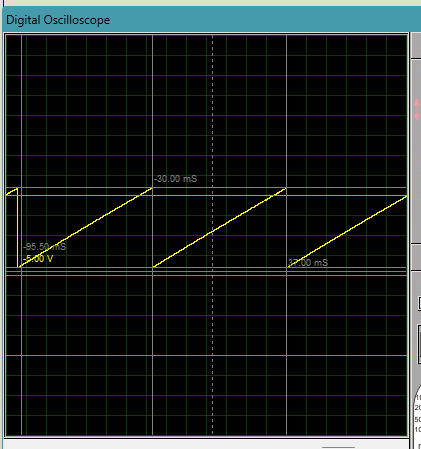
\includegraphics[width=0.9\textwidth]{figures/201.png} % 调整宽度为文本宽度的 80%
    \caption{代码控制效果} %图片标题
    \label{fig:example} % 图片标签,用于引用
\end{figure}

示波器光标测量得:周期为67ms,符合要求;AC挡位测量幅值为5V,符合实验预期。

\begin{figure}[H] % [H] 表示强制当前位置插入
    \centering
    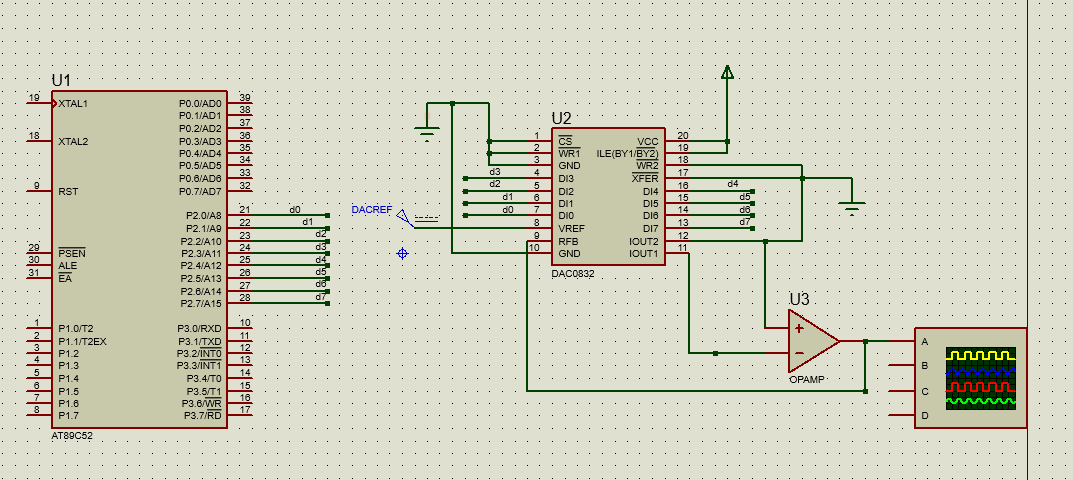
\includegraphics[width=0.9\textwidth]{figures/202.png} % 调整宽度为文本宽度的 80%
    \caption{电路结构} %图片标题
    \label{fig:example} % 图片标签,用于引用
\end{figure}

\section{流程图}


\begin{figure}[H] % [H] 表示强制当前位置插入
        \centering
        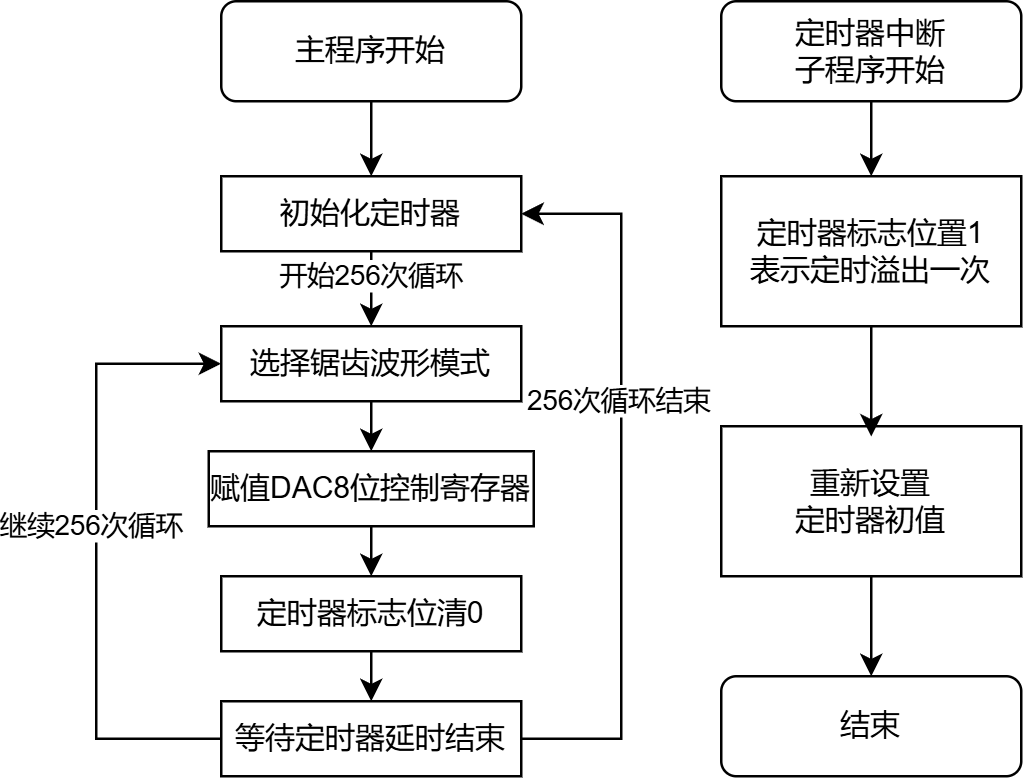
\includegraphics[width=0.9\textwidth]{figures/301.png} % 调整宽度为文本宽度的 80%
        \caption{系统控制流程图} %图片标题
        \label{fig:example} % 图片标签,用于引用
\end{figure}



\section{实验体会}

通过本次锯齿波生成实验,我初步理解了单片机与DAC0832的接口及应用。本实验的收获和体会如下:

\begin{enumerate}
    \item \textbf{DAC原理理解}:实验使我清晰地理解了数模转换的基本原理,掌握了如何通过数字量控制模拟输出。通过编程控制DAC0832,将数字信号转换为模拟电压,从而生成锯齿波形。
    
    \item \textbf{波形生成技术}:学会了利用软件循环和定时器精确控制波形的时间特性。在代码中,通过定时器中断精确控制每个采样点的输出时间,实现了锯齿波的平滑生成。
    
    \item \textbf{定时器应用}:掌握了如何利用定时器中断实现精确的时间控制。为了生成周期为(20+47)ms的锯齿波,需要精确计算定时器的初值,这加深了我对定时器配置和使用的理解。
    
    \item \textbf{系统设计思路}:通过设计不同波形生成函数(锯齿波、三角波和自定义波形),学习了模块化程序设计方法,提高了代码的可读性和复用性。
    
    \item \textbf{波形分析能力}:通过观察实验结果,学习了如何分析实际输出与理论预期之间的差异,理解了实际电子系统中可能出现的误差来源。
    
\end{enumerate}

总体而言,这次实验将理论知识与实际应用紧密结合,不仅加深了我对单片机和数模转换技术的理解,也提升了我的实践动手能力。通过自己编程实现不同波形的生成,增强了我对嵌入式系统设计的信心,为今后学习更复杂的单片机应用奠定了基础。

\end{document}